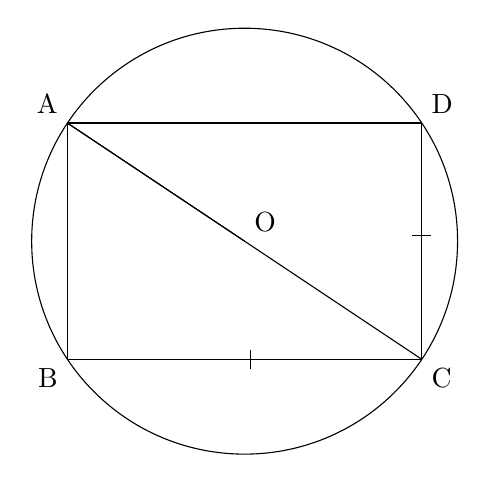
\begin{tikzpicture}[scale=1.5]

% Define points
% A is at top left of rectangle
% B is at bottom left of rectangle
% C is at bottom right of rectangle
% D is at top right of rectangle
% O is the center of the circle (intersection of diagonals)

\coordinate (A) at (0, 2);
\coordinate (B) at (0, 0);
\coordinate (C) at (3, 0);
\coordinate (D) at (3, 2);
\coordinate (O) at (1.5, 1);

% Draw the circle passing through all four corners
% radius = sqrt(1.5^2 + 1^2) = sqrt(3.25) = 1.803
\draw (O) circle (1.803);

% Draw line segment AB (left side of rectangle)
\draw (A) -- (B);

% Draw line segment BC (bottom side of rectangle)
\draw (B) -- (C);

% Draw line segment CD (right side of rectangle)
\draw (C) -- (D);

% Draw line segment DA (top side of rectangle)
\draw (D) -- (A);

% Draw diagonal AC
\draw (A) -- (C);

% Draw line segment AO (from A to center O)
\draw (A) -- (O);

% Draw tick mark on BC (equal length indicator)
\draw (1.55, -0.08) -- (1.55, 0.08);

% Draw tick mark on CD (equal length indicator)
\draw (2.92, 1.05) -- (3.08, 1.05);

% Label point A
\node[above left] at (A) {A};

% Label point B
\node[below left] at (B) {B};

% Label point C
\node[below right] at (C) {C};

% Label point D
\node[above right] at (D) {D};

% Label point O
\node[above right] at (O) {O};

\end{tikzpicture}